%!TEX root = labo.tex
\setcounter{chapter}{1}
\chapter{Frequencies and Channels}

In the \wifi standards, various channels are defined. Two main frequency bands are used, namely 2.4 GHz and 5GHz. \wifi{a} networks use the 5 GHz band, while \wifi{b/g} networks operate in the 2.4 GHz band. In both bands, various ``channels'' have been defined. However, channel separation is not as clean cut as one might expect. In the following setups, you will illustrate this using some simple tests.

\section{Available channels}
\begin{exercise}{Frequencies}

Within the \wifi specification, various channels are defined. Depending on the local authorities (\ac{bipt} in Belgium\cite{bipt}), the list of allowed channels can vary. Using \incommand{iw} you can get the list of available channels.\newline
\remark The wireless drivers we use make a difference between the logical interface (\incommand{wlan0} as we have used it so far) and the actual physical radio interface. All things related to physical characteristics are actually handled by the physical interface, which is called \incommand{phy0} or \incommand{phy1}, respectively.\newline
\begin{enumerate}
	\item  To get a correct overview of which frequencies/channels are available in Belgium, use the command \incommand {iw phy1 info}.
	\item List all frequencies/channels that the \incommand{phy1} interface supports.\newline
	\begin{esolution}
	\end{esolution}
\end{enumerate}

You should observe several frequencies that are marked \emph{disabled}. This indicates that the card supports these frequencies, but cannot use them because of Belgian regulations. Also, several frequencies should be marked with \emph{radar detection}. These can be used, but special mechanisms must be put in place in order to avoid interference with radar installatiuons (e.g. airport radar).

\end{exercise}

\begin{exercise}{Available UA hotspots}
\begin{figure}[h]
	\begin{center}
		
		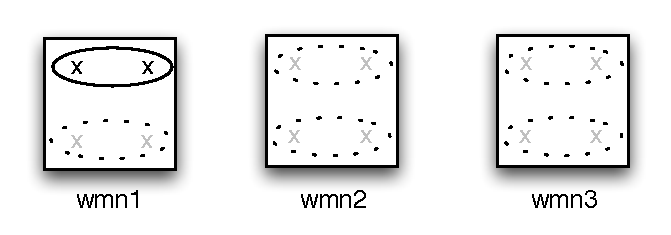
\includegraphics[width=0.5\textwidth]{images/channels1.pdf}
		\caption{Channel separation setup 1} 
		\label{fig:channels1} 
	\end{center}
\end{figure}

\begin{enumerate}
		\item Start by building the setup as illustrated in figure \ref{fig:channels1}. \newline
		\remark Remark that it is not necessary to configure the SSID or channel, but bring up the interface to activate it.
		\item Find out which \acp{ap} are active using \incommand{iw wlan0 scan}. This command provides an interface to list various settings from the \ac{wnic}. The manpage or command line help should be self-explanatory.
		\item Fill in the following table:\newline
		\begin{esolution}
		\end{esolution}
\ifthenelse{\not \boolean{Solutions}}{
		\renewcommand\arraystretch{2.5}
		\setlength\LTleft{0pt}
		\setlength\LTright{0pt}

		\begin{longtable}{@{\extracolsep{\fill}}ccc}
		%{\textwidth}{@{\extracolsep{\fill}}
		\hline
		SSID & Frequency (MHz) & BSS \\
		\hline
		& & \\
		\hline
		& & \\
		\hline
		& & \\
		\hline
		& & \\
		\hline
		\end{longtable}}{}
%		\item \report Write down the exact command used to obtain your results:
%		\begin{esolution}{2}
%		\end{esolution}
	\end{enumerate}
\end{exercise}

\section{Channel Separation}

\begin{exercise}{Channel overhearing} \label{ex:overhearing}
	
	\begin{figure}[h]
		\begin{center}
			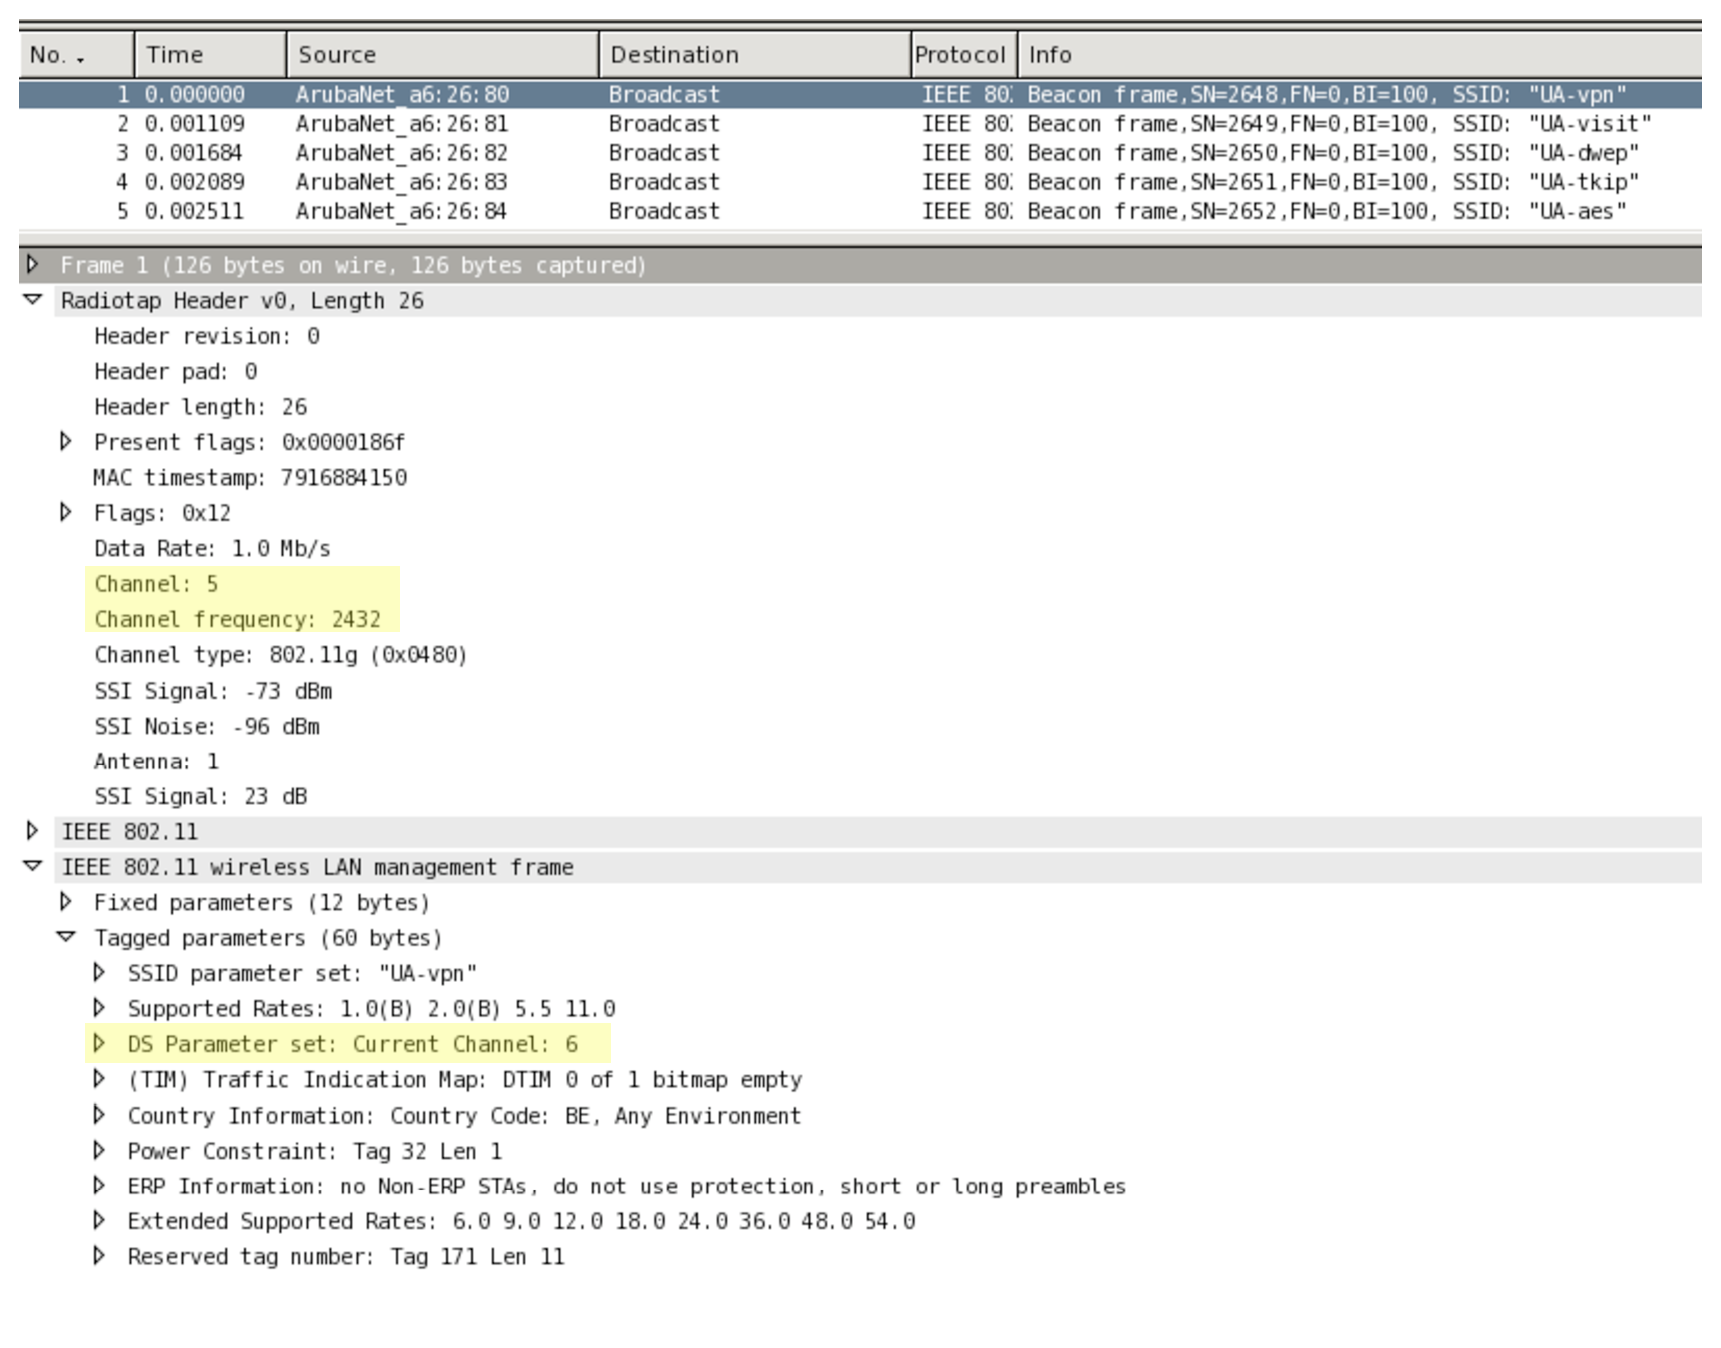
\includegraphics[width=\textwidth]{images/beacon.pdf}
			\caption{Channels in a captured beacon frame.} 
			\label{fig:beacons} 
		\end{center}
	\end{figure}
	
	
In the previous exercise, you made an overview of a lot of \aclp{ap}. The next exercise will illustrate the channel overhearing. The information about which channel an \ac{ap} is working on, is provided in the beacon frames the \ac{ap} periodically transmits. In figure \ref{fig:beacons}, a Wireshark\cite{wireshark} screen shot shows a beacon frame. The Radiotap header indicates the frame was received on channel 5, while the beacon's content shows the \ac{ap} sending this beacon only operates at channel 6. Channels are thus not cleanly separated.  In the next exercise you'll create an overview of the channel overhearing.

\begin{figure}[h!]
		\begin{center}
			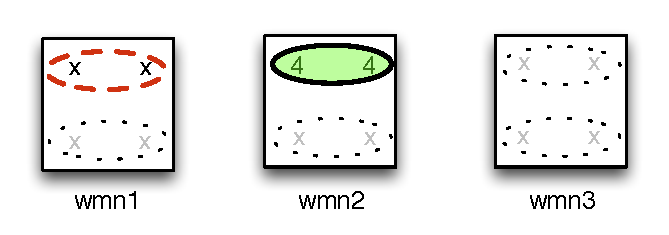
\includegraphics[width=0.5\textwidth]{images/channels2.pdf}
			\caption{Setup for exercise \ref{ex:overhearing}.} 
			\label{fig:channels2} 
		\end{center}
\end{figure}
	
	\begin{enumerate}
		\item Start from the setup as shown in figure \ref{fig:channels2}. \newline
		\remark Note that the \ac{ap} should be configured in channel 4 from the b/g range. To be able to do this, you should change the line \verb!hw_mode=a! to \verb!hw_mode=b! in the hostapd.conf file.
		\item On \ac{sta}1, on every channel, make a capture \file{chanID.pcap}.\newline
		\item Use the following wireshark display filter to only show beacons:\newline
		\command{wlan.fc.type\_subtype == 8}
		\item Fill out the following table using the obtained information.\newline
		\begin{esolution}
		\end{esolution}
		

\ifthenelse{\not \boolean{Solutions}}{
\begin{longtable}{@{\extracolsep{\fill}}c|l}	
	Selected channel & Observed channels in received beacons \\
	\hline
	1&\\\hline
	2&\\\hline
	3&\\\hline
	4&\\\hline
	5&\\\hline
	6&\\\hline
	7&\\\hline
	8&\\\hline
	9&\\\hline
	10&\\\hline
	11&\\\hline
\end{longtable}	}{}
		\end{enumerate}
\end{exercise}

\begin{figure}[h!]
	\begin{center}
		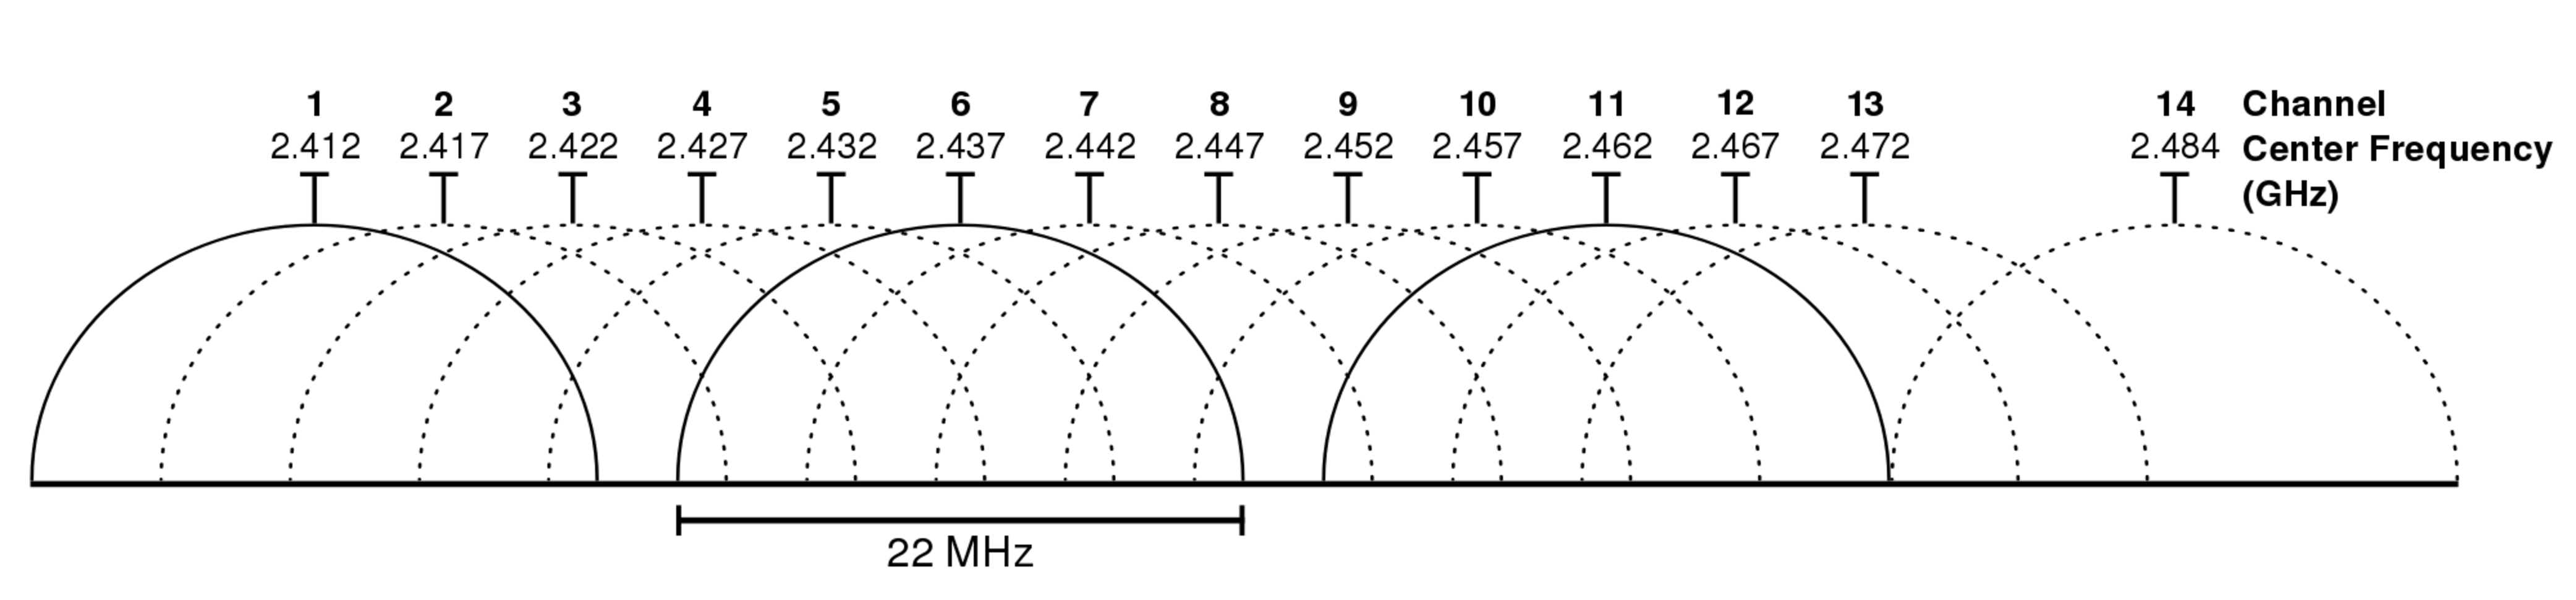
\includegraphics[width=\textwidth]{images/bgchannels.pdf}
		\caption{2.4 GHz channels} 
		\label{fig:channel_separation} 
	\end{center}
\end{figure}

From this exercise, it should be clear that the channels within the \wifi{b/g} range are not strictly separated.  Figure \ref{fig:channel_separation}\footnote{By Michael Gauthier, Wireless Networking in the Developing World [CC-BY-SA-3.0 (http://creativecommons.org/licenses/by-sa/3.0)], via Wikimedia Commons} gives you an idea why: the consecutive channels overlap to a certain extent. Therefore, a careful channel planning is crucial in building and deploying wireless networks on these frequencies. In the next exercise, we will take a look at the channel separation in the \wifi{a} band.

\begin{exercise}{Channel separation in \wifi{a}}\label{ex:separation}
	
	\begin{enumerate}
		\item Now, change the \ac{ap} so that it is on channel \verb!x!.
		\item Using \incommand{tcpdump} as in the previous exercise, find out in which channels \wifi{a} the beacons of this \ac{ap} can be seen. Save your traces in \file{chanID.pcap}.\newline
		\begin{esolution}
		\end{esolution}
	\end{enumerate}
	
\end{exercise}

\section{Using the Wireless Channel}

\begin{figure}[h]
		\begin{center}
			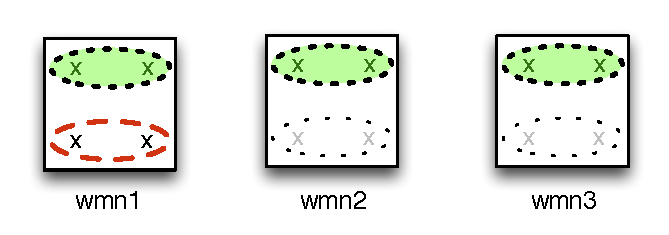
\includegraphics[width=0.5\textwidth]{images/adhoc2.pdf} 
			\caption{Basic ad-hoc network.}
			\label{fig:ad-hoc2} 
		\end{center}
	\end{figure}
	
\begin{exercise}{Beacons}

In the next few exercises, we will again use an ad-hoc network setup. It is best to reboot the devices before proceeding.
\begin{enumerate}
	\item Create the network setup as shown in figure \ref{fig:ad-hoc2}. Perform the following commands on all three stations. Substitute \incommand{nodeNumber} with a different number (e.g. 1, 2 and 3) on each node.\newline
		\command{\prompt{wmn} iw dev wlan0 set type ibss}
		\command{\prompt{wmn} ip addr add fc00:\acs{gid}::nodeNumber/64 dev wlan0}
		\command{\prompt{wmn} ifconfig wlan0 up}
		\command{\prompt{wmn} iw dev wlan0 ibss join \acs{wmn}-\acs{gid}-A <frequency>}
	\item Put interface wlan1 of \ac{sta}1 in monitor mode on the same frequency.\newline
		\command{\prompt{\ac{sta}1} iw dev wlan1 set type monitor}
		\command{\prompt{\ac{sta}1} ifconfig wlan1 up}
		\command{\prompt{\ac{sta}1} iw dev wlan1 set freq <frequency>}
	\item Check if all stations can reach each other.
	\item Perform a \incommand{tcpdump} on the monitor interface. Save it to \file{\acs{sta}1.pcap}. Let it run for a few seconds and then stop the trace.
	\item In your trace file, you should observe beacon frames. Carefully inspect one of the beacon frames in this trace and compare it to a beacon frame captured in the previous exercise (exercise \ref{ex:separation}). Give the packet IDs of the beacon frames you are comparing and identify the differences in the management frame part.\newline
	\begin{esolution}
	\end{esolution}
	\item Start a new trace on the monitor interface and save it to \file{STA1.pcap}.
	\item While the trace is running, perform two ping tests. You may perform the simultaneously, but it will be easier to answer the next question if you perform them consecutively.\newline
	\command{\prompt{\ac{sta}2} ping6 -c 5 fc00:\acs{gid}::3}
	\command{\prompt{\ac{sta}3} ping6 -s 1400 -c 5 fc00:\acs{gid}::1}
	\item Open your trace file and filter out the beacon frames with the following display filter: \verb#!(wlan.fc.type_subtype == 0x08)#. Apart from the data frames, which kind of frames do you observe?\newline
	\begin{esolution}
	\end{esolution}
	\item Explain the purpose of those frames.\newline
	\begin{esolution}
	\end{esolution}
\end{enumerate}
\end{exercise}

\begin{exercise}{\ac{rts}/\ac{cts}}

For this exercise, you will study the \ac{rts}/\ac{cts} mechanism. This mechanism will clear the channel for each transmission, minimizing the chance of collisions in the channel. A threshold value is used to determine if \ac{rts}/\ac{cts} should be used. Larger packets will receive \ac{rts}/\ac{cts} protections while smaller packet will not. Using \ac{rts}/\ac{cts} for small packets adds a lot of overhead and hence degrades performance.

\begin{enumerate}
	\item Start from the setup as for the previous exercise.
	\item The \ac{rts}/\ac{cts} threshold will be set with \incommand{iwconfig wlan0 rts 1000}. Perform this command on all nodes.
	\item Performing the same \incommand{ping6} commands as in the previous exercise. Start a capture session on the monitor interface and save it to \file{STA1.pcap}.
	\item You should observe \ac{rts}/\ac{cts} packets. Which packets are protected by this mechanism? Give an example (packet ID).\newline
	\begin{esolution}
	\end{esolution}
	\item Compare an \ac{rts} and \ac{cts} frame. How do they differ? Illustrate using frames from your last trace file.
	\begin{esolution}
	\end{esolution}
\end{enumerate}

As you can see in the \ac{rts}/\ac{cts} frames, they do not contain any information about the network on which they are transmitted. The \ac{rts}/\ac{cts} is meant to avoid collisions on the wireless medium, so any node that receives a \ac{cts} frame is required to remain silent for the duration included in the \ac{cts} frame. The only exception, for obvious reasons, is the node to which the \ac{cts} frame is sent. Capturing \ac{rts}/\ac{cts} frames (or acknowledgement frames) on a certain channel is always a good indication that some activity is going on in that channel, even if it is impossible to overhear the actual data transmission.
\end{exercise}

\section{\wifi{n}}


Until now, we have only used the \acp{wnic} in \wifi{a} or b/g mode. ``b'' is the oldest mode. ``g'' improves upon ``b'' by offering significantly higher maximal throughput (54 Mbps versus 11 Mbps) .``a'' operates at different frequencies and offers the same throughput as ``g''.

Another mode of operation is called ``n''. \wifi{n} is an amendment to the \wifi standard in order to improve throughput over both ``a'' and ``g''. It operates at both frequency bands and is defined for bit rates up to 600 Mbps, but very few setups will be able to obtain these speeds.

\wifi{n} can use different optimizations, such as the \ac{mimo} principle, 40 MHz wide channels (versus 20 MHz in \wifi{a/b/g}), and frame aggregation to improve throughput. The following exercise will demonstrate that \wifi{n} channels can indeed be twice as wide as those in \wifi{a}, and thus interfere with adjacent \wifi{a} channels.

\begin{exercise}{\wifi{n}}

\begin{figure}[h]
		\begin{center}
			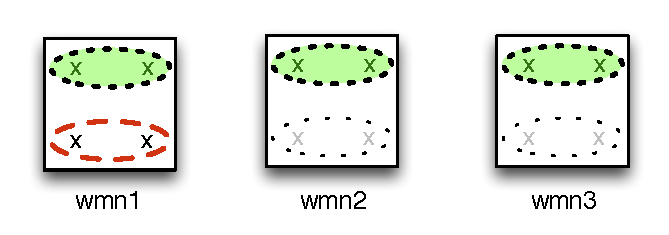
\includegraphics[width=0.5\textwidth]{images/adhoc2.pdf} 
			\caption{\wifi{n} ad-hoc network.}
			\label{fig:ad-hoc-n} 
		\end{center}
	\end{figure}

\stress{As this exercise will use both channels allocated to the mobile and wireless lab, two groups cannot perform this exercise at the same time! Check if no other group is currently working on this course!} 

\begin{enumerate}
	\item Reboot all devices. In order to enable \wifi{n} mode without any problems, we will start from a blank setup.
	\item After they have been rebooted, perform the following on all devices in order to create an ad-hoc network with \wifi{n} support in the 5 GHz band:\newline
		\command{\prompt{\ac{sta}} iw dev wlan0 set type ibss}
		\command{\prompt{\ac{sta}} ip addr add fc00:\acs{gid}::nodeNumber/64 dev wlan0}
		\command{\prompt{\ac{sta}} ifconfig wlan0 up}
		\command{\prompt{\ac{sta}} iw dev wlan0 ibss join wmn-\acs{gid}-A 5180 HT20}
	\item Check that all nodes can reach each other.
	\item Set up a monitor interface on channel 36 (5180 MHz) on \ac{sta}1.
	\item Start a trace on the monitor interface and save it to \file{\acs{sta}1.pcap}.
	\item Start a ping from \ac{sta}2 to \ac{sta}3 and from \ac{sta}3 to \ac {sta}1. Like before, use different ping sizes:\newline
		\command{\prompt{\ac{sta}2} ping6 -c 5 fc00:\acs{gid}::3}
		\command{\prompt{\ac{sta}3} ping6 -s 1400 -c 5 fc00:\acs{gid}::1}
	\item Filter out the beacon frames from your trace. Do you observe packets from both ping sessions? Did you see all packets from these sessions? Why or why not?\newline
	\begin{esolution}
	\end{esolution}
	\item Set the monitor interface to channel 40 (5200 MHz).
	\item Perform the same ping test again, but now save your trace to \file{\acs{sta}1.pcap}.
	\item Did you capture any packets?\newline
	\begin{esolution}
	\end{esolution}
\end{enumerate}

	
\end{exercise}

\begin{exercise}{40 MHz channels}

In the previous exercise, we enabled \wifi{n}, but we did not enable 40 MHz wide channels yet. We will do that now.
\begin{enumerate}
	\item Deconfigure all \incommand{wlan0} interfaces.\newline
	\command{\prompt{\ac{sta}} iw dev wlan0 ibss leave}
	\item Now, create an ad-hoc network that uses 40 MHz wide channels:\newline
	\command{\prompt{\ac{sta}} iw dev wlan0 ibss join wmn-0-A 5180 HT40+}
	\item As in the previous exercise, set the monitor interface of \ac{sta}1 on channel 36 and perform a capture while sending both pings. Save it to \file{\acs{sta}1.36.pcap}.
	\item Do the same again, but this time monitor channel 40.\newline Save your trace in \file{\acs{sta}1.40.pcap}.
	\item Do you observe any different behaviour in the trace file on channel 36, compared to the previous exercise?\newline
	\begin{esolution}
	\end{esolution}
	\item In the trace file on channel 40, which packets have you captured? Why?\newline
	\begin{esolution}
	\end{esolution}
\end{enumerate}
\end{exercise}
